% -------------------------------------------------------------------
{
\begin{figure*}[hbt]
% \newcommand{\figWidth}{.45\linewidth}
% \newcommand{\clipfig}[1]{\psclip{\psframe[linecolor=white](0.,1.)(5.4,4.85)}\epsfig{#1}\endpsclip}
\psset{xunit=1.cm,yunit=1.cm,runit=1.cm}
% 
\newcommand{\figWidtha}{7.5cm}
\newcommand{\clipfig}[2]{\clipFig{#1}{#2}{.0}{1.}{0.05}{.9}}
% 
\begin{center}
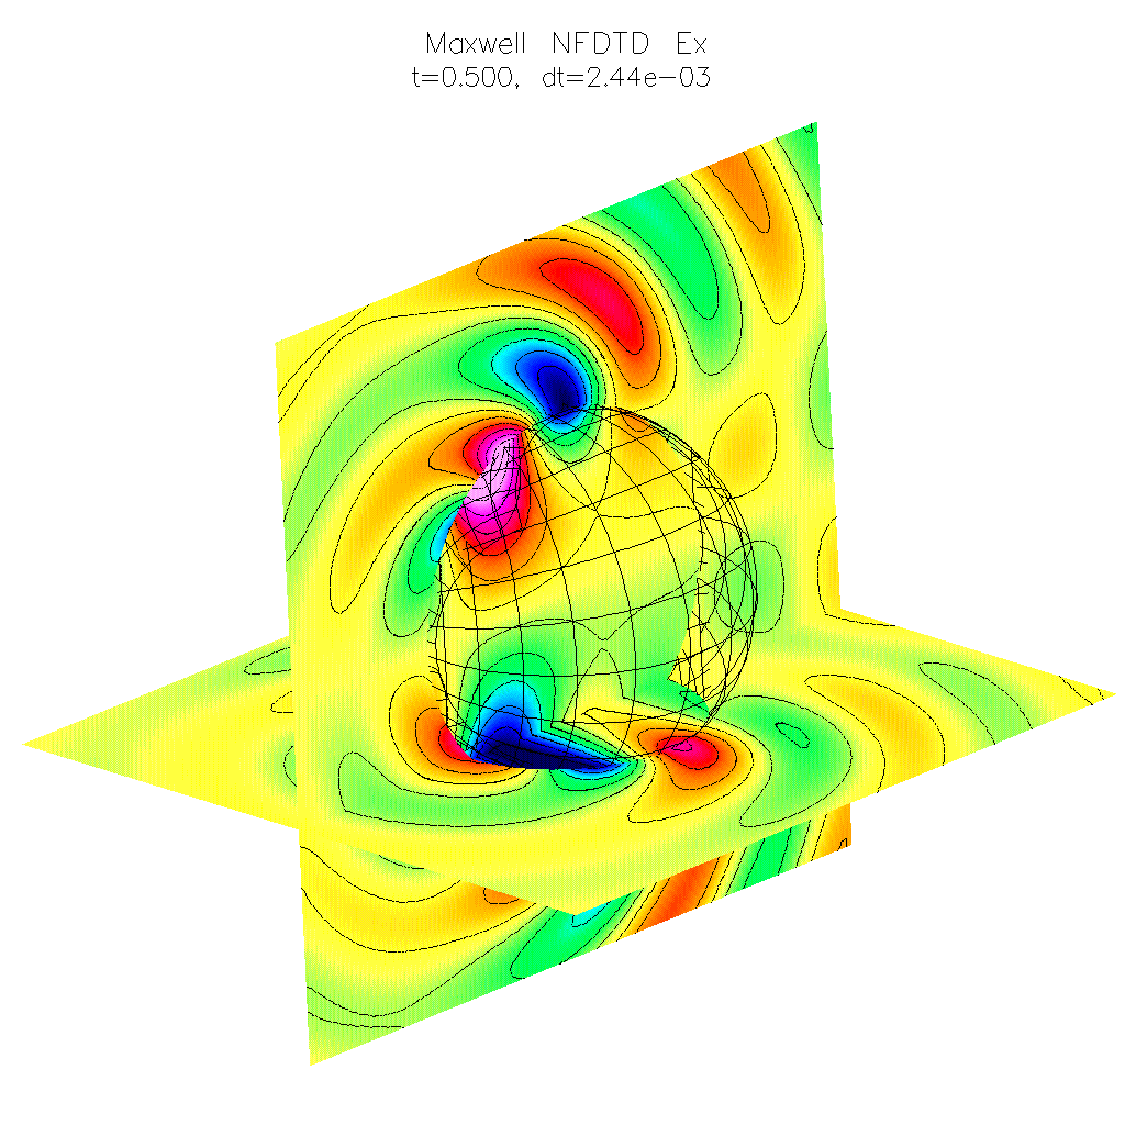
\includegraphics[width=\figWidtha]{figures/scatDielectricSphereEx}
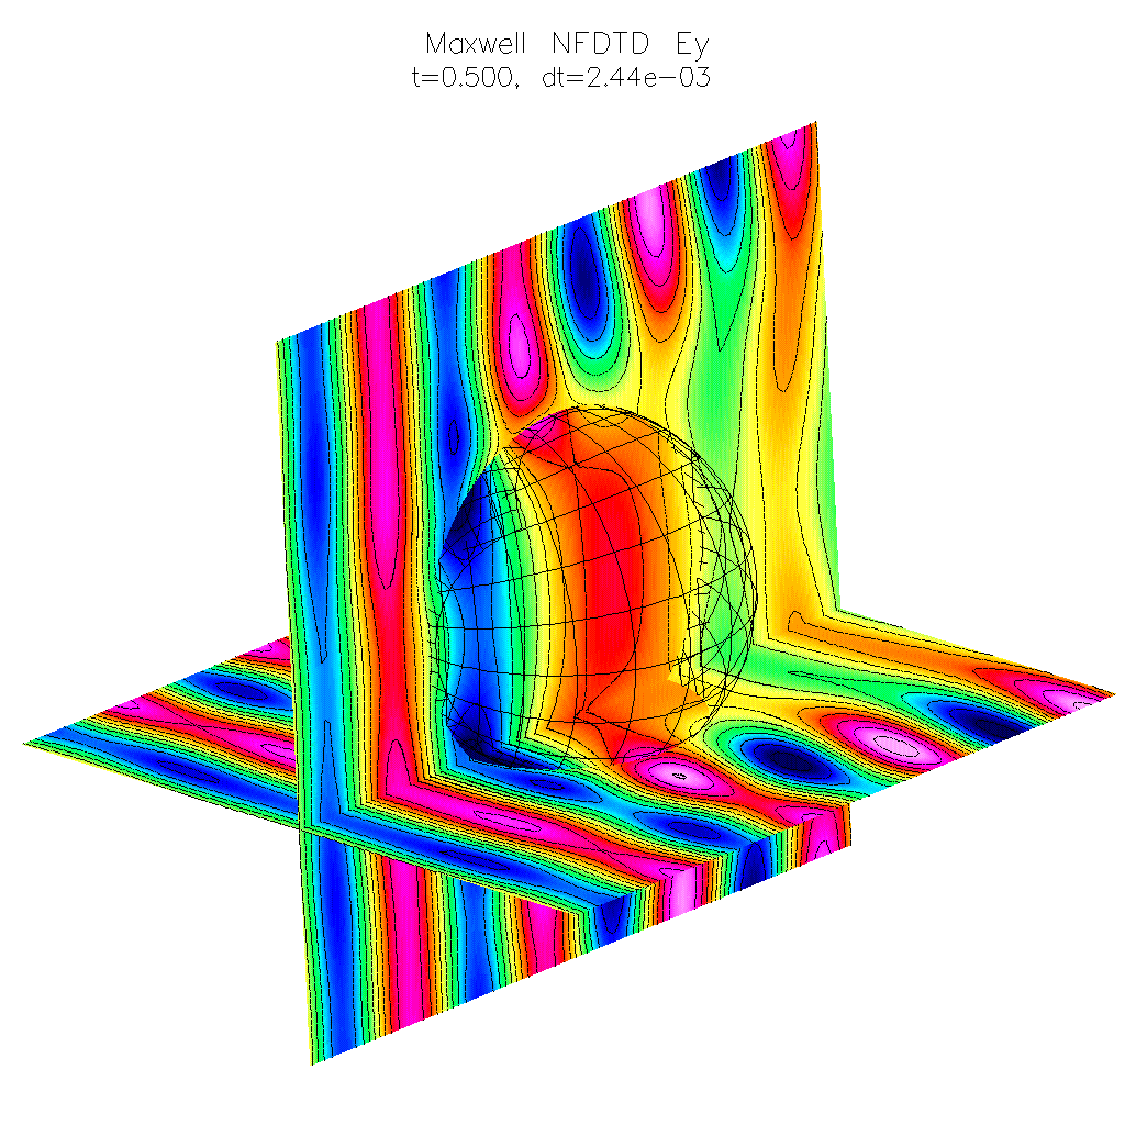
\includegraphics[width=\figWidtha]{figures/scatDielectricSphereEy}
%- \begin{pspicture}(0,0)(14.2,5.2)
%- % \rput( 3.2,9.){\clipfig{dielectricCyl44-1p0-Ex.ps}{\figWidth}}
%- % \rput( 9.5,9.){\clipfig{dielectricCyl44-1p0-Ey.ps}{\figWidth}}
%- \rput( 3.2,2.6){\clipfig{figures/scatDielectricSphereEx}{\figWidtha}}
%- \rput(10.5,2.6){\clipfig{figures/scatDielectricSphereEy}{\figWidtha}}
%- % 
%- % \rput[l](.70,11.5){\psframebox*[fillstyle=solid,fillcolor=mediumgoldenrod]{$E_X$}}
%- % \rput[l](7.0,11.5){\psframebox*[fillstyle=solid,fillcolor=mediumgoldenrod]{$E_y$}}
%- \rput[l](1.3,4.6){\psframebox*[fillstyle=solid,fillcolor=mediumgoldenrod]{$E_x$}}
%- \rput[l](8.5,4.6){\psframebox*[fillstyle=solid,fillcolor=mediumgoldenrod]{$E_y$}}
%- % 
%- % \psline[linewidth=1.pt]{->}(7,-.8)(7.5,.9)
%- % turn on the grid for placement
%- % \psgrid[subgriddiv=2]
%- %
%- \end{pspicture}
\end{center}
\caption{Scattering of a plane wave by a dielectric sphere at $t=.5$ with $k_x=1$, $\eps_1=.25$ (inside), $\eps_2=1$ (outside). 
The fields for $E_x$ and $E_y$ are shown.}
\label{fig:scatDielectricSphereFig}
\end{figure*}
}
